 \chapter{Samples based CdTe}
\label{chap:appendix2}
\textit{In this annex the results obtained from the modifications made on HgCdTe and CdTe samples are discussed. Mechanical modifications on the surface and silver evaporations were performed with the objective of understanding the behavior of a metal on a semiconductor. The idea of modifying the surfaces by evaporating was proposed, due to the intention of understanding in a fundamental way the novel materials known as topological insulators and given the particular phenomena that were presented in the HgCdTe quantum wells under considerations that will be addressed in this annex, the proposal is to study CdTe surfaces with Ag evaporations with the help of the e-beam coupled in the vacuum chamber.}
\vfill
\minitoc
\newpage

\allowdisplaybreaks

The objective of the study by means of differential reflectance of the surface of HgCdT and of the materials of the CdTe family and especially CdTe with Ag evaporation is to reconstruct or to make a similarity of the surface position of the topological insulators, these materials that show properties of conductors in the surface and insulators in the bulk. 

In first approximation this was implemented with the objective to know the surface of quantum wells of HgCdTe which show this behavior and it is due to the fact that in the walls the domains are stressed by the fact of the growth by MBE of this type of materials, for us a first approximation was to recreate in HgCdTe in bulk, small zones that would show stress and that we could monitor them by RDS, so the following was done: 

\begin{enumerate}
	\item In the HgCdTe sample using diamond paste we started to make in a preferential addition this carving or these surface modifications.
	\item Evaporations of Ag which is a metal and we expect a similar behavior and that this will help us to compare what is the evolution when performing these treatments. 
\end{enumerate}
\section{Samples Descriptions}
\vspace{-1cm}

\newcolumntype{C}{>{\centering\arraybackslash}p{80mm}}% a centered fixed-width-column
\begin{table}[H]
	\centering
	\begin{tabular}{lC}
		\hline
		\hline
		&  Description\\
		\hline
		Sample 01 & CdTe \\
		Sample 02 & HgCdTe\\
		Sample 03 & HgCdTe\\
		Sample 04 & HgCdTe con superficie tallada \\
		Sample 05 & HgCdTe con superficie evaporada\\
		Sample 06 & CdZnTe\\
		\hline
		\hline
	\end{tabular}
	\caption{Samples studied from the $CdTe$ family}
	\label{tab:CH 3 Section 3.1 Photodectors materials}
\end{table}

\begin{figure}[htp] 
	\centering
	
	\subfloat[data a]{%
	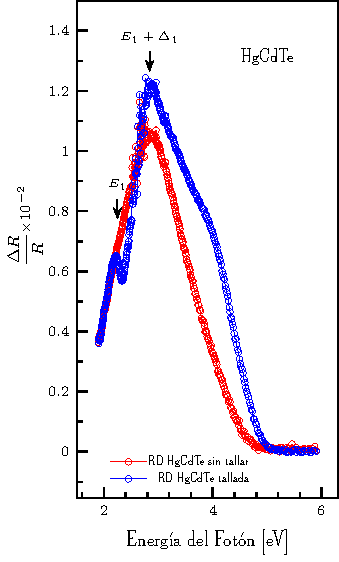
\includegraphics[width=0.4\textwidth]{FIGURES/Anexo-CdTe/hgcdte-tallada.pdf}%
	\label{fig:a}%
	}
	\subfloat[data b]{\vspace{1.05cm}
	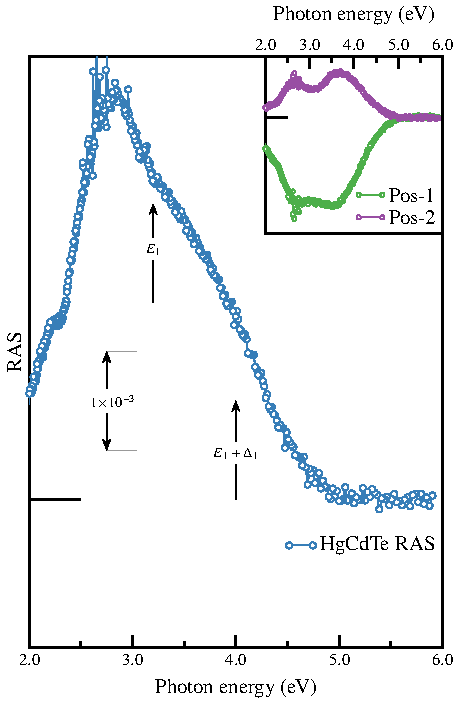
\includegraphics[width=0.4\textwidth]{FIGURES/Anexo-CdTe/image04.pdf}%
	\label{fig:b}%
	}
	
	\caption{all the data}
\end{figure}


%%Pares de imagenes Funcion dielectrica - RD %% 
\subsection{CdTe}
\begin{figure}[htp] 
	\centering
	
	\subfloat[data a]{%
	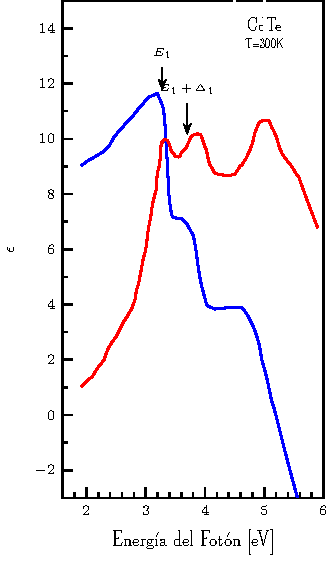
\includegraphics[width=0.4\textwidth]{FIGURES/Anexo-CdTe/fd-CdTe.pdf}%
	\label{fig:a}%
	}
	\subfloat[data b]{\vspace{1.05cm}
	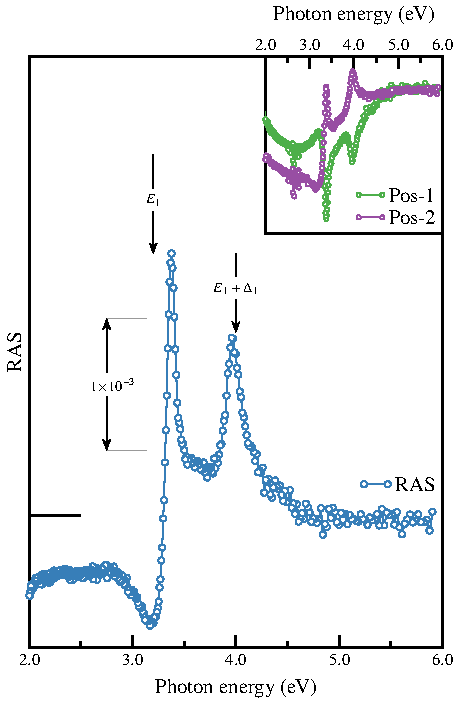
\includegraphics[width=0.4\textwidth]{FIGURES/Anexo-CdTe/image02.pdf}%
	\label{fig:b}%
	}
	\caption{all the data}
\end{figure}

\subsection{ZnTe}
\begin{figure}[htp] 
	\centering
	
	\subfloat[data a]{%
	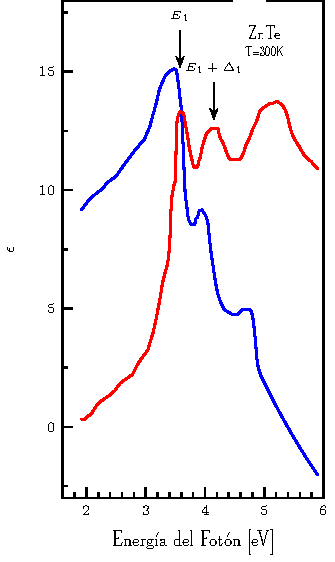
\includegraphics[width=0.4\textwidth]{FIGURES/Anexo-CdTe/fd-ZnTe.pdf}%
	\label{fig:a}%
	}
	\subfloat[data b]{\vspace{1.05cm}
	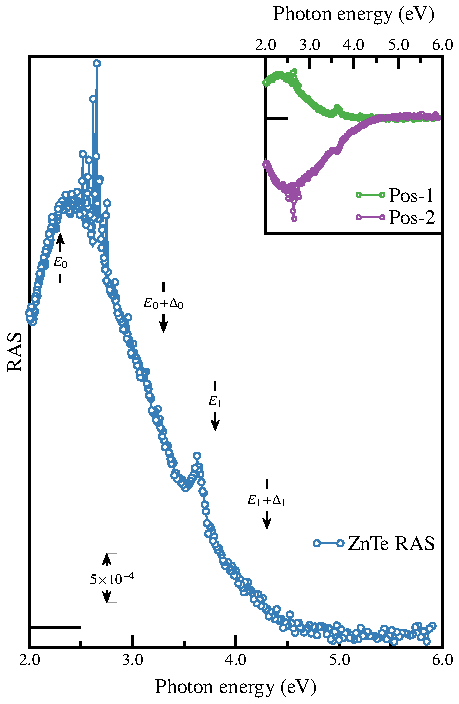
\includegraphics[width=0.4\textwidth]{FIGURES/Anexo-CdTe/image06.pdf}%
	\label{fig:b}%
	}
	\caption{all the data}
\end{figure}



\subsection{CdZnTe}
En este apartado 
\begin{figure}[htp] 
	\centering
	
	\subfloat[data a]{%
	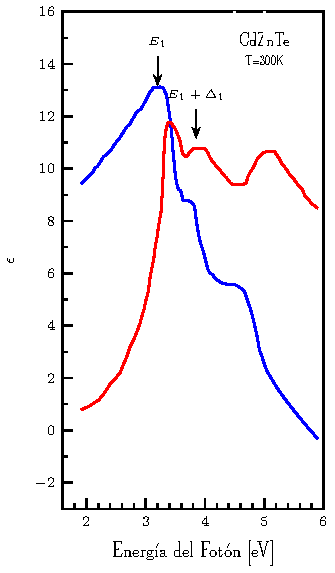
\includegraphics[width=0.4\textwidth]{FIGURES/Anexo-CdTe/fd-CdZnTe.pdf}%
	\label{fig:a}%
	}
	\subfloat[data b]{\vspace{1.05cm}
	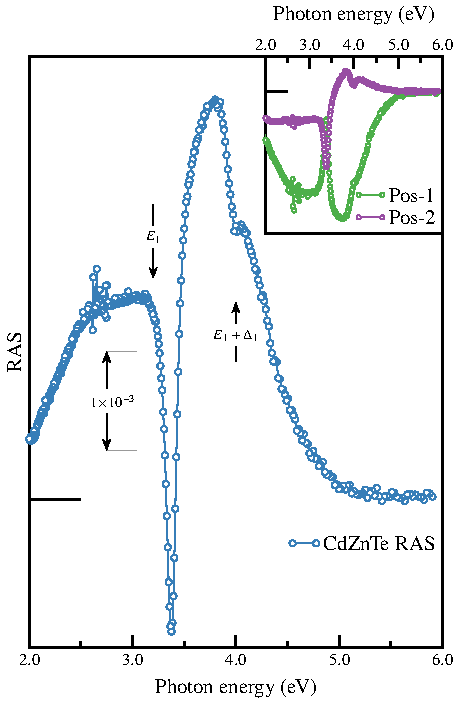
\includegraphics[width=0.4\textwidth]{FIGURES/Anexo-CdTe/image03.pdf}%
	\label{fig:b}%
	}
	\caption{all the data}
\end{figure}

\begin{figure}
	\centering
	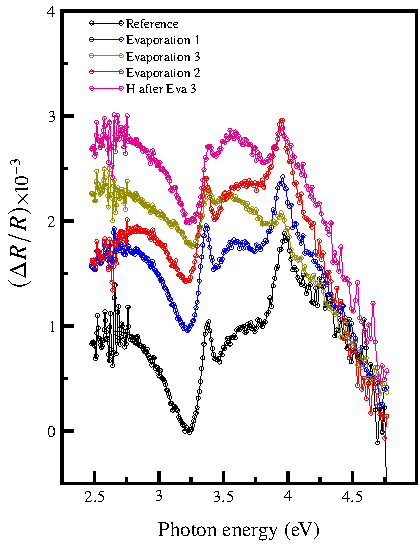
\includegraphics[width=0.65\linewidth]{FIGURES/Anexo-CdTe/rds-evaporated-cdte-5.pdf}
	\caption{Carbon allotrope timeline}
	\label{fig:introfig32}
\end{figure}

\section{Results an Conclusions}
\vspace{-1cm}

The evaporations were carried out with the e-beam performing the process of emptying the Ag material in the crucible, likewise the necessary treatment was given to the crucible so that it was in optimal cleaning conditions since the material previously contained was gadolinium. 

One of the disadvantages when performing the evaporation of the material is that in literature this type of process comments that in several cases do not show a complete homogeneity in the evaporation of the same, this may be because the surface is not necessarily heated while evaporating, the temperature is not adequate and can be evaporated by drops, clusters, nanoparticles and even in so-called islands, in various works such as those of ...... comments that under the conditions of heating the substrate and the distance at which it is located is quite optimal or likely to cover a wide area, so several evaporations were performed on the same sample and likewise several cases were monitored from the clean surface to the last evaporation and a reheated (this part is done because the area is more stable in terms of the surface), in conclusion the realiados processes were as follows.  